% !TEX encoding = UTF-8
% !TEX TS-program = pdflatex
% !TEX root = ../Tesi.tex
% !TEX spellcheck = it-IT

\clearpage

\section{Attore utente pubblico}
%
% Figura: casi d'uso dell'attore utente pubblico
%
\begin{figure}[h]
	\centering
	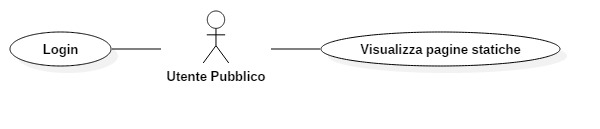
\includegraphics[width=1\textwidth]
	{immagini/uc-utente-pubblico}
	
	\caption{Casi d'uso dell'attore utente pubblico}
\end{figure}


%
% Caso d'uso: Visualizza pagine statiche
%
\subsection{Caso d'uso: Visualizza pagine statiche}

	\subsubsection*{Descrizione}
	Questa funzionalità permette all'utente pubblico di visualizzare tutte le pagine richieste con contenuto non dinamico.
	
	\subsubsection*{Attori coinvolti}
	Utente pubblico, partecipazione attiva, richiedendo la visualizzazione delle pagine.
	
	\subsubsection*{Pre-condizioni}
	Nessuna precondizione, in quanto non serve uno stato particolare per visualizzare una pagina statica.
	
	\subsubsection*{Post-condizioni}
	Nessuna postcondizione, in quanto la visualizzazione di una pagina statica non altera lo stato dell'applicazione.
	
	\subsubsection*{Flusso principale}
	
	\begin{enumerate}
		
		\item
		Richiesta di qualsiasi pagina che abbia contenuto statico da parte dell'utente pubblico
		
		\item
		Risposta del server con la pagina statica richiesta da parte dell'utente pubblico;
		
	\end{enumerate}
	
	\subsubsection*{Flussi alternativi}
	Non presenti.

%
% Caso d'uso: Effettua login
%
\subsection{Caso d'uso: Effettua login}

	\subsubsection*{Descrizione}
	Questa funzionalità permette all'utente pubblico di farsi riconoscere dal sistema, accedendo quindi alle funzionalità che sono a lui riservate.
	
	\subsubsection*{Attori coinvolti}
	Utente pubblico, partecipazione attiva dell'attore che passa da Utente Pubblico ad Amministratore o Gestore squadra o Arbitro.
	
	\subsubsection*{Pre-condizioni}
	Compilazione del modulo di login.
	
	\subsubsection*{Post-condizioni}
	L'utente passa da attore Utente Pubblico ad Amministratore o Gestore squadra o Arbitro.
	
	\subsubsection*{Flusso principale}
	
	\begin{enumerate}
		
		\item
		L'utente pubblico seleziona la voce ``Login'' nella pagina in cui si trova;
		
		\item
		L'utente pubblico compila il modulo inserendo la propria email e la propria password;
		
		\item
		L'utente pubblico seleziona la voce ``Accedi'';
		
		\item
		Il sistema effettua verifica se le informazioni inserite nel campo email sono corrette dal punto di vista sintattico inviando all'utente pubblico, in caso di errore, una notifica con l'errore riscontrato;
		
		\item
		Il sistema dopo aver ricevuto i dati il server controlla se nella base dati è presente un utente con indirizzo email e password ricevuti;
		
		\item
		Se le informazioni esistono sulla base dati l'utente pubblico viene riconosciuto dal sistema. L'utente visualizza il suo nome e cognome con un messaggio di benvenuto che lo informa della sua tipologia. L'utente selezionando la voce ``MyHome'' visualizza la propria home page e un menù con tutte le operazioni che può eseguire sul sistema.
		
	\end{enumerate}
	
	\subsubsection*{Flussi alternativi}
	Nel caso di inserimento di email e password non presenti nel database vengono notificate all'utente pubblico le possibili cause di errore.
	
	\subsection*{Diagramma delle attività}
	Il diagramma delle attività per il caso d'uso ``Effettua login'' è illustrato nella figura \vref{ad-login}.
	
	
	%
	% Figura: diagramma delle attività relativo al login di un utente
	%
	\begin{figure}[h]
		\centering
		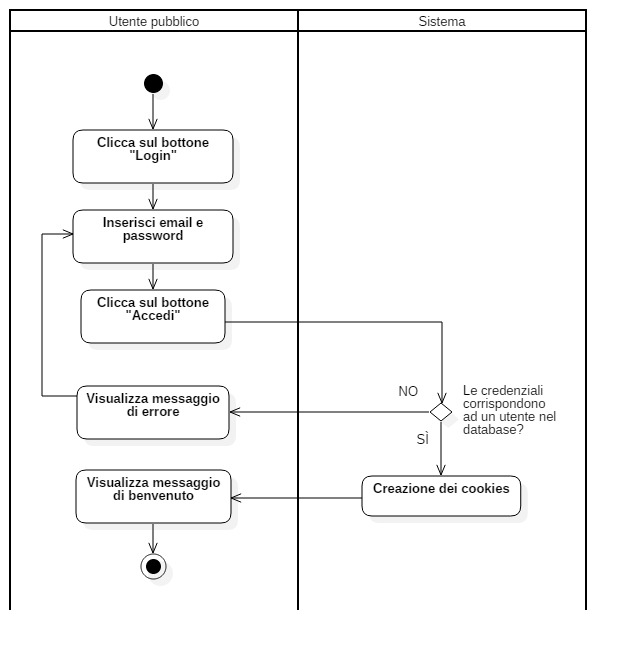
\includegraphics[width=0.8\textwidth]
		{immagini/ad-login}
		
		\caption{Diagramma delle attività del login di un utente pubblico}
		\label{ad-login}
	\end{figure}